\section{Casi d'uso}
    \subsection{Introduzione}
    In questa sezione vengono descritti i casi d'uso che descrivono tutte le funzionalità che \emph{HD Viz} dovrà offrire all'utente.
    \subsection{Attori dei casi d'uso}
    Per utilizzare \emph{HD Viz} non è necessario essere autenticati.
    \subsubsection{Attori}
    \begin{description}
        \item[Utente] \hfill \\Generico utente che accede ad \emph{HD Viz} per creare una visualizzazione a partire dai dati che possiede.
    \end{description}
    \subsection{UC1 - Inserimento dei dati }
\label{uc1}

    \begin{figure}[htbp]
        \centering
        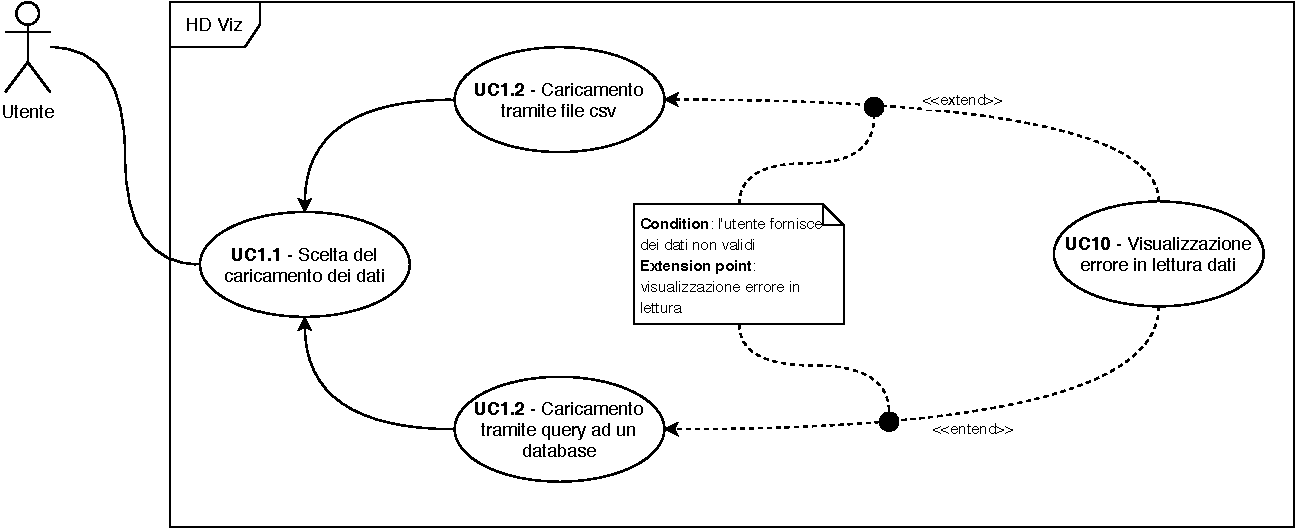
\includegraphics[width=1.0\textwidth]{source/sections/casi-uso/diagrams/uc1.pdf}
        \caption{UC1 - Inserimento dei dati}
        % \label{fig:uc1}
    \end{figure}
    
    \begin{itemize}
    \item \textbf{Attore}: utente;
    \item \textbf{Descrizione}: l'utente carica i dati per ottenere una visualizzazione;
    \item \textbf{Precondizione}:
    \begin{itemize}
        \item il sistema è funzionante e raggiungibile;
        \item l'utente accede alla pagina dell'applicazione.
    \end{itemize}
    \item \textbf{Postcondizione}: i dati sono stati caricati correttamente come matrice $N\times M$;
    \item \textbf{Scenario Principale}: 
        \begin{enumerate}
            \item l'utente accede alla pagina dell'applicazione;
            \item l'utente sceglie come caricare i dati (\hyperref[uc1.1]{UC1.1}):
                \begin{enumerate}
                    \item l'utente ha scelto di ricavare i dati caricando un file csv;
                    \item l'utente ha scelto di ricavare i dati tramite una query a un database.
                \end{enumerate}
        \end{enumerate}  
    \item \textbf{Estensioni}:
        \begin{enumerate}
            \item l'utente inserisce dei dati non validi o non nel formato corretto:
                \begin{enumerate}
                    \item fallisce l'inserimento dei dati;
                    \item viene visualizzato un messaggio di errore in lettura dei dati (\hyperref[uc10]{UC10}).
                \end{enumerate}
        \end{enumerate}  
    \item \textbf{Generalizzazioni}:
        \begin{enumerate}
            \item l'utente sceglie come caricare i dati:
                \begin{enumerate}
                    \item caricando un file csv (\hyperref[uc1.2]{UC1.2});
                    \item tramite una query a un database (\hyperref[uc1.3]{UC1.3}).
                \end{enumerate}
        \end{enumerate}  
    \end{itemize}
    
    %%%
    \subsubsection{UC1.1 - Scelta del caricamento dei dati}
    \label{uc1.1}
    
    \begin{itemize}
    \item \textbf{Attore}: utente;
    \item \textbf{Descrizione}: l'utente sceglie come caricare i dati;
    \item \textbf{Precondizione}:
    \begin{itemize}
        \item il sistema è funzionante e raggiungibile;
        \item l'utente accede alla pagina dell'applicazione.
    \end{itemize}
    \item \textbf{Postcondizione}: l'utente ha fatto la scelta;
    \item \textbf{Scenario Principale}: 
        \begin{enumerate}
            \item l'utente sceglie come caricare i dati in base alle proprie esigenze.
        \end{enumerate}
    \end{itemize}
    
    %%%
    \subsubsection{UC1.2 - Caricamento tramite file csv}
    \label{uc1.2}
    
    \begin{itemize}
    \item \textbf{Attore}: utente;
    \item \textbf{Descrizione}: l'utente sceglie di caricare i dati tramite un file csv;
    \item \textbf{Precondizione}:
    \begin{itemize}
        \item il sistema è funzionante e raggiungibile;
        \item l'utente accede alla pagina dell'applicazione;
        \item l'utente è in possesso di un file csv contenete i dati.
    \end{itemize}
    \item \textbf{Input}: file csv contenente i dati da visualizzare;
    \item \textbf{Postcondizione}: l'utente ha caricato il suo file csv come matrice $N\times M$;
    \item \textbf{Scenario Principale}: 
        \begin{enumerate}
            \item l'utente ha scelto di inserire i file tramite un file csv;
            \item tramite l'apposito bottone sceglie il file.
        \end{enumerate}
        \item \textbf{Estensioni}:
        \begin{enumerate}
            \item l'utente inserisce dei dati non validi o non nel formato corretto:
                \begin{enumerate}
                    \item fallisce l'inserimento dei dati;
                    \item viene visualizzato un messaggio di errore in lettura dei dati. (\hyperref[uc10]{UC10}):
                \end{enumerate}
        \end{enumerate}  
    \end{itemize}

    
    %%%
    \subsubsection{UC1.3 - Caricamento tramite query ad un database}
    \label{uc1.3}
    
    Il caricamento tramite database è descritto in modo generale. L'analisi più approfondita di questo requisito sarà stesa durante la prossima revisione, dopo aver fissato una \emph{Technology Baseline}. In ogni caso sarà possibile ricavare i dati da almeno un tipo di database SQL e da almeno un tipo di database NoSQL.
    
    \begin{itemize}
    \item \textbf{Attore}: utente;
    \item \textbf{Descrizione}: l'utente sceglie di caricare i dati tramite tramite query ad un database;
    \item \textbf{Precondizione}:
    \begin{itemize}
        \item il sistema è funzionante e raggiungibile;
        \item l'utente accede alla pagina dell'applicazione;
        \item l'utente può collegarsi ad un database (possiede le credenziali).
    \end{itemize}
    \item \textbf{Postcondizione}: l'utente si è collegato al database e ha recuperato i dati tramite query come matrice $N\times M$;
    \item \textbf{Scenario Principale}: 
        \begin{enumerate}
            \item l'utente ha scelto di caricare i dati tramite tramite query ad un database in cui può collegarsi;
            \item inserisce le credenziali, e scrive la sua query per ricavare i dati.
        \end{enumerate}
        \item \textbf{Estensioni}:
        \begin{enumerate}
            \item l'utente inserisce dei dati non validi o non nel formato corretto:
                \begin{enumerate}
                    \item fallisce l'inserimento dei dati;
                    \item viene visualizzato un messaggio di errore in lettura dei dati (\hyperref[uc10]{UC10}).
                \end{enumerate}
        \end{enumerate}  
    \end{itemize}

    
    \pagebreak
    \subsection{UC2 - Scelta della visualizzazione }
\label{uc2}

    % \includegraphics{}
    \begin{itemize}
    \item \textbf{Attore}: Utente
    \item \textbf{Descrizione}: L'utente all'interno dell'applicazione sceglie la visualizzazione che vuole ottenere
    \item \textbf{Precondizione}:
    \begin{itemize}
        \item Il sistema è funzionante e raggiungibile
        \item L'utente accede alla pagina dell'applicazione
    \end{itemize}
    \item \textbf{Postcondizione}: L'utente ha scelto quale visualizzazione vuole ottenere
    \item \textbf{Scenario Principale}: 
        \begin{enumerate}
            \item L'utente seleziona la visualizzazione tra quelle disponibili
        \end{enumerate}  
    \item \textbf{Generalizzazioni}:
        \begin{enumerate}
            \item L'utente seleziona una delle seguenti visualizzazioni
                \begin{enumerate}
                    \item Scatter Plot Matrix (\hyperref[uc2.1]{UC2.1})
                    \item Heatmap (\hyperref[uc2.2]{UC2.2})
                    \item Correlation Heatmap (\hyperref[uc2.3]{UC2.3})
                    \item Force Field (\hyperref[uc2.4]{UC2.4})
                    \item Linear Projection (\hyperref[uc2.5]{UC2.5})
                    \item Parallel Coordinates (\hyperref[uc2.6]{UC2.6})
                \end{enumerate}
        \end{enumerate}  
    \end{itemize}
    
    %%%
    \subsubsection{UC2.1 - Scatter Plot Matrix}
    \label{uc2.1}
    
    \begin{itemize}
    \item \textbf{Attore}: Utente
    \item \textbf{Descrizione}: L'utente sceglie la visualizzazione \emph{Scatter Plot Matrix}
    \item \textbf{Precondizione}:
    \begin{itemize}
        \item Il sistema è funzionante e raggiungibile
        \item L'utente accede alla pagina dell'applicazione
    \end{itemize}
    \item \textbf{Postcondizione}: L'utente sceglie Scatter Plot Matrix come visualizzazione
    \item \textbf{Scenario Principale}: 
        \begin{enumerate}
            \item L'utente sceglie Scatter Plot Matrix come visualizzazione
        \end{enumerate}
    \end{itemize}
    
    %%%
    \subsubsection{UC2.2 - Heatmap}
    \label{uc2.2}
    
    \begin{itemize}
    \item \textbf{Attore}: Utente
    \item \textbf{Descrizione}: L'utente sceglie la visualizzazione \emph{Heatmap}
    \item \textbf{Precondizione}:
    \begin{itemize}
        \item Il sistema è funzionante e raggiungibile
        \item L'utente accede alla pagina dell'applicazione
    \end{itemize}
    \item \textbf{Postcondizione}: L'utente sceglie Heatmap come visualizzazione
    \item \textbf{Scenario Principale}: 
        \begin{enumerate}
            \item L'utente sceglie Heatmap come visualizzazione
        \end{enumerate}
    \end{itemize}
    
    %%%
    \subsubsection{UC2.3 - Correlation Heatmap}
    \label{uc2.3}
    
    \begin{itemize}
    \item \textbf{Attore}: Utente
    \item \textbf{Descrizione}: L'utente sceglie la visualizzazione \emph{Correlation Heatmap}
    \item \textbf{Precondizione}:
    \begin{itemize}
        \item Il sistema è funzionante e raggiungibile
        \item L'utente accede alla pagina dell'applicazione
    \end{itemize}
    \item \textbf{Postcondizione}: L'utente sceglie Correlation Heatmap come visualizzazione
    \item \textbf{Scenario Principale}: 
        \begin{enumerate}
            \item L'utente sceglie Correlation Heatmap come visualizzazione
        \end{enumerate}
    \end{itemize}
    
    %%%
    \subsubsection{UC2.4 - Force Field}
    \label{uc2.4}
    
    \begin{itemize}
    \item \textbf{Attore}: Utente
    \item \textbf{Descrizione}: L'utente sceglie la visualizzazione \emph{Force Field}
    \item \textbf{Precondizione}:
    \begin{itemize}
        \item Il sistema è funzionante e raggiungibile
        \item L'utente accede alla pagina dell'applicazione
    \end{itemize}
    \item \textbf{Postcondizione}: L'utente sceglie Force Field come visualizzazione
    \item \textbf{Scenario Principale}: 
        \begin{enumerate}
            \item L'utente sceglie Force Field come visualizzazione
        \end{enumerate}
    \end{itemize}
    
    %%%
    \subsubsection{UC2.5 - Linear Projection}
    \label{uc2.5}
    
    \begin{itemize}
    \item \textbf{Attore}: Utente
    \item \textbf{Descrizione}: L'utente sceglie la visualizzazione \emph{Linear Projection}
    \item \textbf{Precondizione}:
    \begin{itemize}
        \item Il sistema è funzionante e raggiungibile
        \item L'utente accede alla pagina dell'applicazione
    \end{itemize}
    \item \textbf{Postcondizione}: L'utente sceglie Linear Projection come visualizzazione
    \item \textbf{Scenario Principale}: 
        \begin{enumerate}
            \item L'utente sceglie Linear Projection come visualizzazione
        \end{enumerate}
    \end{itemize}
    
    %%%
    \subsubsection{UC2.6 - Parallel Coordinates}
    \label{uc2.6}
    
    \begin{itemize}
    \item \textbf{Attore}: Utente
    \item \textbf{Descrizione}: L'utente sceglie la visualizzazione \emph{Parallel Coordinates}
    \item \textbf{Precondizione}:
    \begin{itemize}
        \item Il sistema è funzionante e raggiungibile
        \item L'utente accede alla pagina dell'applicazione
    \end{itemize}
    \item \textbf{Postcondizione}: L'utente sceglie Parallel Coordinates come visualizzazione
    \item \textbf{Scenario Principale}: 
        \begin{enumerate}
            \item L'utente sceglie Parallel Coordinatescome visualizzazione
        \end{enumerate}
    \end{itemize}
    
  

    \pagebreak
    \subsection{UC3 - Scelta delle Labels}
\label{uc3}

    \begin{figure}[htbp]
        \centering
        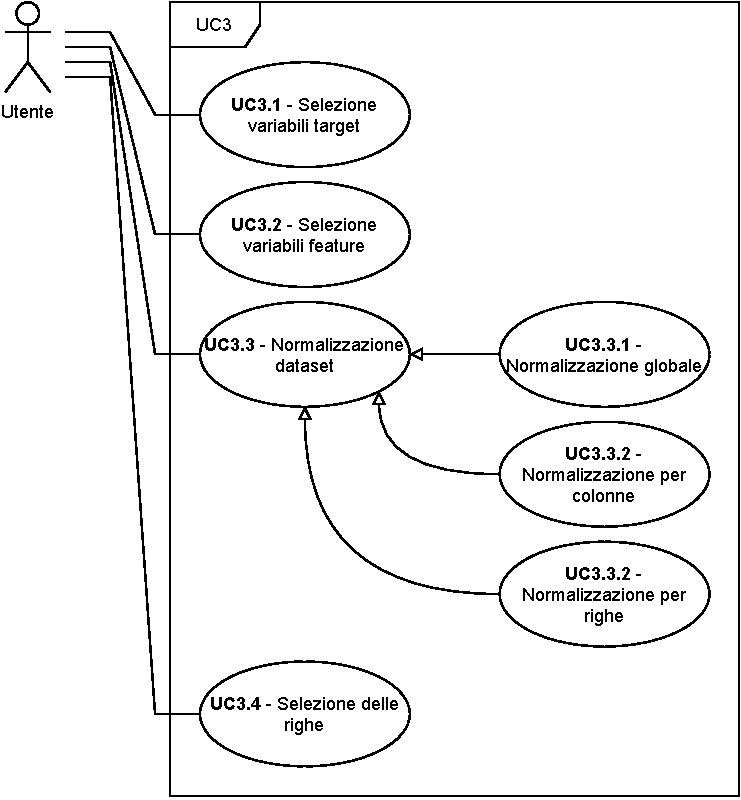
\includegraphics[width=0.5\textwidth]{source/sections/casi-uso/diagrams/uc3.pdf}
        \caption{UC3 - Scelta delle Labels}
        \label{fig:uc3}
    \end{figure}


    \begin{itemize}
    \item \textbf{Attore}: Utente
    \item \textbf{Descrizione}: Tra le dimensioni (colonne della matrice) del dataset caricato possono essere presenti delle labels, l'applicazione offre un meccanismo tramite cui l'utente può selezionare queste tipo di features e separarle dalle features numeriche che invece compongono le coordinate del dato $n$-dimensionale.
    \item \textbf{Precondizione}:
    \begin{itemize}
        \item Eseguito l'upload del dataset come matrice $N\times M$ (\hyperref[uc2]{UC2}).
        \item Selezionata una tra le visualizzazioni Scatter Plot Matrix (\hyperref[uc2.1]{UC2.1}), Force Field (\hyperref[uc2.4]{UC2.4}) Linear Projection (\hyperref[uc2.5]{UC2.5})
    \end{itemize}
    \item \textbf{Postcondizione}: Le features selezionate verranno considerate dal sistema come labels.
    \item \textbf{Scenario Principale}: 
    \begin{enumerate}
        \item L'utente visualizza le features del dataset.
        \item Seleziona le features del dato che ritiene essere delle labels.
    \end{enumerate}  
    \end{itemize}
    
    \subsubsection{UC3.1 - Assegnazione delle classi di visualizzazione alle Labels}
    \label{uc3.1}
    \begin{itemize}
    \item \textbf{Attore}: Utente
    \item \textbf{Descrizione}: L'utente decide di assegnare dei diversi modi per distinguere un punto nel grafico, assegnando una classe di visualizzazione (colore, forma, size) ad ogni label, in questo modo risulta più semplice per l'analista vedere dei pattern nella visualizzazione del grafico.
    \item \textbf{Precondizione}:
    \begin{itemize}
        \item Eseguito l'upload del dataset come matrice $N\times M$ (\hyperref[uc2]{UC2}).
        \item Selezionato una tra le visualizzazioni Scatter Plot Matrix (\hyperref[uc2.1]{UC2.1}), Force Field (\hyperref[uc2.4]{UC2.4}) Linear Projection (\hyperref[uc2.5]{UC2.5}).
        \item Nel dataset, almeno una feature è stata selezionata come label.
    \end{itemize}
    \item \textbf{Postcondizione}: Al variare del valore della etichetta $X$, i punti visualizzati assumono un diverso attributo della classe assegnata a quest'ultima.
    \item \textbf{Scenario Principale}: 
    \begin{enumerate}
        \item L'utente visualizza tutte le labels selezionate.
        \item L'utente associa ad ogni label una classe di visualizzazione.
    \end{enumerate}  
    \end{itemize}
    \pagebreak
    \subsection{UC4 - Selezione manuale delle Features}
\label{uc4}
 %   \includegraphics{}
    \begin{itemize}
    \item \textbf{Attore}: Utente
    \item \textbf{Descrizione}: L'utente può scartare le features di un dato che non è interessato a visualizzare.
    \item \textbf{Precondizione}: 
     \begin{itemize}
        \item Eseguito l'upload del dataset come matrice $N\times M$ (\hyperref[uc1]{UC1}).
        \item Selezionato un tipo di visualizzazione (\hyperref[uc2]{UC2}).
    \end{itemize}
    \item \textbf{Postcondizione}: La matrice contiene $M-i$ colonne, dove $i$ è il numero di features che l'utente ha scartato.
    \item \textbf{Scenario Principale}: 
    \begin{enumerate}
        \item L'utente visualizza le features del dataset, che corrispondono alle colonne della matrice
        \item L'utente scarta le features a cui non è interessato
    \end{enumerate}
    \item \textbf{Generalizzazioni}:
        \begin{enumerate}
            \item Selezione manuale delle features per Scatter Plot Matrix (\hyperref[uc4.1]{UC4.1})
        \end{enumerate}
    \end{itemize}
    
    \subsubsection{UC4.1 - Selezione manuale delle Features per Scatter Plot Matrix}
    \label{uc4.1}
    \begin{itemize}
    \item \textbf{Attore}: Utente
    \item \textbf{Descrizione}: L'utente può selezionare al massimo 5 features da visualizzare.
    \item \textbf{Precondizione}: 
     \begin{itemize}
        \item Eseguito l'upload del dataset come matrice $N\times M$ (\hyperref[uc1]{UC1}).
        \item Selezionato Scatter Plot Matrix come visualizzazione (\hyperref[uc2.1]{UC2.1}).
    \end{itemize}
    \item \textbf{Postcondizione}: La matrice contiene al massimo 5 colonne cioè le features che l'utente ha selezionato.
    \item \textbf{Scenario Principale}: 
    \begin{enumerate}
        \item L'utente visualizza le features del dataset, che corrispondono alle colonne della matrice
        \item L'utente sceglie le features che è intenzionato a visualizzare
    \end{enumerate}  
    \end{itemize}
    \pagebreak
    \subsection{UC5 - Calcolo matrice di distanza}
    \label{uc5}
    
    \begin{figure}[htbp]
        \centering
        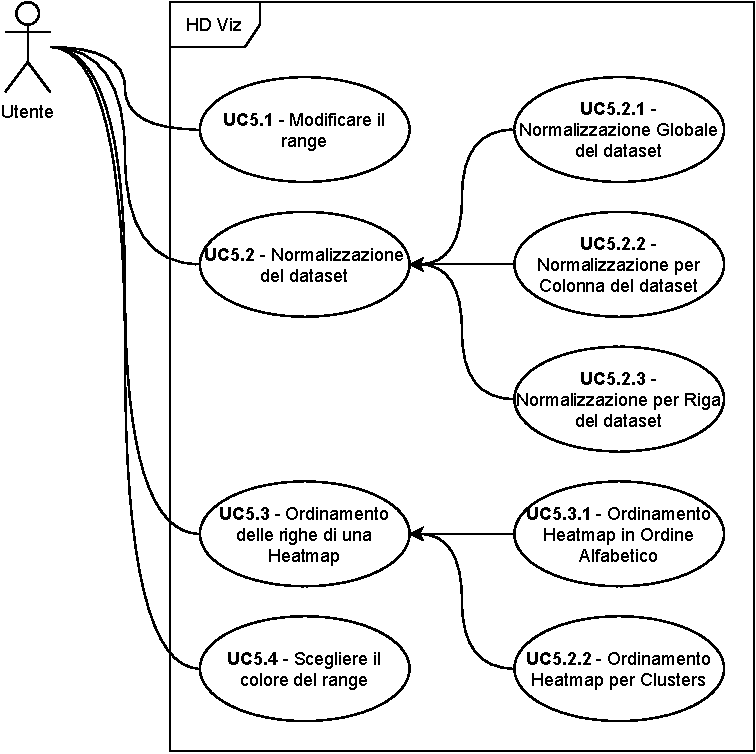
\includegraphics[width=0.9\textwidth]{source/sections/casi-uso/diagrams/uc5.pdf}
        \caption{UC5 - Calcolo matrice di distanza}
        \label{fig:uc5}
    \end{figure}
    
    \begin{itemize}
    \item \textbf{Attore}: utente;
    \item \textbf{Descrizione}: data una matrice $N \times M$ viene calcolata la distanza tra ogni riga e viene restituita all'utente una matrice di distanza N x N dove ${x_i}_j$ è la distanza tra la riga $i$ e la riga $j$ della matrice di partenza;
    \item \textbf{Precondizione}: 
    \begin{itemize}
        \item eseguito l'upload del dataset come matrice $N\times M$ (\hyperref[uc1.1]{UC1.1});
        \item selezionato Heatmap o Force Field come visualizzazione (\hyperref[uc2.1.2]{UC2.1.2} o \hyperref[uc2.1.4]{UC2.1.4}).
    \end{itemize}  
    \item \textbf{Postcondizione}: calcolata matrice di distanza $N \times N$ dove ${x_i}_j$ è la distanza tra la riga $i$ e la riga $j$ della matrice di partenza;
    \item \textbf{Scenario Principale}: 
    \begin{enumerate}
        \item l'utente seleziona il calcolo della matrice di distanza corrispondente al dataset caricato;
        \item l'utente seleziona la distanza (\hyperref[uc5.1]{UC5.1}).
    \end{enumerate}
    \end{itemize}
    
    \subsubsection{UC5.1 - Selezione distanza}
    \label{uc5.1}
    \begin{itemize}
    \item \textbf{Attore}: utente;
    \item \textbf{Descrizione}: l'utente sceglie la distanza da utilizzare per l'elaborazione del dataset;
    \item \textbf{Precondizione}: 
    \begin{itemize}
        \item eseguito l'upload del dataset come matrice $N\times M$ (\hyperref[uc1.1]{UC1.1}).
        \item selezionato Heatmap o Force Field come grafico su cui visualizzare il dataset (\hyperref[uc2.1.2]{UC2.1.2} o \hyperref[uc2.1.4]{UC2.1.4}).
        \item selezionato calcola matrice di distanza (\hyperref[uc5]{UC5}).
    \end{itemize}  
    \item \textbf{Postcondizione}: l'utente ha scelto la distanza da utilizzare;
    \item \textbf{Scenario Principale}: 
    \begin{enumerate}
        \item l'utente seleziona la distanza tra quelle disponibili.
    \end{enumerate}
    \item \textbf{Generalizzazioni}:
        \begin{enumerate}
            \item l'utente seleziona una delle seguenti distanze:
                \begin{enumerate}
                    \item Euclidea (\hyperref[uc5.1.1]{UC5.1.1});
                    \item Manhattan (\hyperref[uc5.1.2]{UC5.1.2}).
                \end{enumerate}
        \end{enumerate}  
    \end{itemize}
    
    \paragraph{UC5.1.1 - Distanza euclidea}
    \label{uc5.1.1}
    \begin{itemize}
    \item \textbf{Attore}: utente;
    \item \textbf{Descrizione}: l'utente sceglie la distanza \emph{Euclidea};
    \item \textbf{Precondizione}: 
    \begin{itemize}
        \item eseguito l'upload del dataset come matrice $N\times M$ (\hyperref[uc1.1]{UC1.1});
        \item selezionato Heatmap o Force Field come visualizzazione (\hyperref[uc2.1.2]{UC2.1.2} o \hyperref[uc2.1.4]{UC2.1.4}).
        \item selezionato calcola matrice di distanza (\hyperref[uc5]{UC5}).
    \end{itemize}  
    \item \textbf{Postcondizione}: l'utente ha scelto la distanza euclidea;
    \item \textbf{Scenario Principale}: 
    \begin{enumerate}
        \item l'utente ha scelto la distanza euclidea.
    \end{enumerate}
    \end{itemize}
    
    \paragraph{UC5.1.2 - Distanza di Manhattan}
    \label{uc5.1.2}
    \begin{itemize}
    \item \textbf{Attore}: utente;
    \item \textbf{Descrizione}: l'utente sceglie la distanza di \emph{Manhattan};
    \item \textbf{Precondizione}: 
    \begin{itemize}
        \item eseguito l'upload del dataset come matrice $N\times M$ (\hyperref[uc1.1]{UC1.1});
        \item selezionato Heatmap o Force Field come visualizzazione (\hyperref[uc2.1.2]{UC2.1.2} o \hyperref[uc2.1.4]{UC2.1.4}).
        \item selezionato calcola matrice di distanza (\hyperref[uc5]{UC5}).
    \end{itemize}  
    \item \textbf{Postcondizione}: l'utente ha scelto la distanza di Manhattan;
    \item \textbf{Scenario Principale}: 
    \begin{enumerate}
        \item l'utente ha scelto la distanza di Manhattan.
    \end{enumerate}
    \end{itemize}

    \pagebreak
        \subsection{UC6 - Calcolo Matrice di Distanza}
    % \includegraphics{}
    \begin{itemize}
    \item \textbf{Attore}: Utente
    \item \textbf{Descrizione}: Data una matrice $N \times M$ viene calcolata la distanza tra ogni riga e viene restituita all'utente una matrice di distanza N x N dove ${x_i}_j$ è la distanza tra la riga i e la riga j della matrice di partenza.
    \item \textbf{Precondizione}: 
    \begin{itemize}
        \item Eseguito l'upload del dataset come matrice $N\times M$ (\hyperref[uc1]{UC1}).
        \item Selezionato Heatmap o Force Field come visualizzazione (\hyperref[uc2.2]{UC2.2} o \hyperref[uc2.4]{UC2.4}).
    \end{itemize}  
    \item \textbf{Postcondizione}: Calcolata matrice di distanza $N \times N$ dove ${x_i}_j$ è la distanza tra la riga $i$ e la riga $j$ della matrice di partenza.
    \item \textbf{Scenario Principale}: 
    \begin{enumerate}
        \item L'utente seleziona il calcolo della matrice di distanza corrispondente al dataset caricato
        \item L'utente seleziona la distanza (\hyperref[uc6.1]{UC6.1})
    \end{enumerate}  
    \item \textbf{Inclusioni}:
        \begin{enumerate}
                \item \begin{enumerate}
                    \item Scelta dell'algoritmo di distanza da utilizzare (\hyperref[uc6.1]{UC6.1})
                \end{enumerate}
        \end{enumerate} 
    \end{itemize}
    
    \subsubsection{UC6.1 - Selezione distanza}
    \label{uc6.1}
    \begin{itemize}
    \item \textbf{Attore}: Utente
    \item \textbf{Descrizione}: L'utente sceglie la distanza da utilizzare durante l'elaborazione dati
    \item \textbf{Precondizione}: 
    \begin{itemize}
        \item Eseguito l'upload del dataset come matrice $N\times M$ (\hyperref[uc1]{UC1}).
        \item Selezionato Heatmap o Force Field come visualizzazione (\hyperref[uc2.2]{UC2.2} o \hyperref[uc2.4]{UC2.4}).
    \end{itemize}  
    \item \textbf{Postcondizione}: L'utente ha scelto la distanza da utilizzare
    \item \textbf{Scenario Principale}: 
    \begin{enumerate}
        \item L'utente seleziona la distanza tra quelle disponibili
    \end{enumerate}
    \item \textbf{Generalizzazioni}:
        \begin{enumerate}
            \item L'utente seleziona una delle seguenti distanze
                \begin{enumerate}
                    \item Euclidea (\hyperref[uc6.1.1]{UC6.1.1})
                    \item Manhattan (\hyperref[uc6.1.2]{UC6.1.2})
                \end{enumerate}
        \end{enumerate}  
    \end{itemize}
    
    \paragraph{UC6.1.1 - Distanza Euclidea}
    \label{uc6.1.1}
    \begin{itemize}
    \item \textbf{Attore}: Utente
    \item \textbf{Descrizione}: L'utente sceglie la distanza \emph{Euclidea}
    \item \textbf{Precondizione}: 
    \begin{itemize}
        \item Eseguito l'upload del dataset come matrice $N\times M$ (\hyperref[uc1]{UC1}).
        \item Selezionato Heatmap o Force Field come visualizzazione (\hyperref[uc2.2]{UC2.2} o \hyperref[uc2.4]{UC2.4}).
    \end{itemize}  
    \item \textbf{Postcondizione}: L'utente ha scelto la distanza euclidea
    \item \textbf{Scenario Principale}: 
    \begin{enumerate}
        \item L'utente ha scelto la distanza euclidea
    \end{enumerate}
    \end{itemize}
    
    \paragraph{UC6.1.2 - Distanza di Manhattan}
    \label{uc6.1.2}
    \begin{itemize}
    \item \textbf{Attore}: Utente
    \item \textbf{Descrizione}: L'utente sceglie la distanza di \emph{Manhattan}
    \item \textbf{Precondizione}: 
    \begin{itemize}
        \item Eseguito l'upload del dataset come matrice $N\times M$ (\hyperref[uc1]{UC1}).
        \item Selezionato Heatmap o Force Field come visualizzazione (\hyperref[uc2.2]{UC2.2} o \hyperref[uc2.4]{UC2.4}).
    \end{itemize}  
    \item \textbf{Postcondizione}: L'utente ha scelto la distanza di Manhattan
    \item \textbf{Scenario Principale}: 
    \begin{enumerate}
        \item L'utente ha scelto la distanza di Manhattan
    \end{enumerate}
    \end{itemize}
    \pagebreak
    \subsection{UC7 - Selezione algoritmo di riduzione delle componenti}
    \label{uc7}
    
    \begin{figure}[htbp]
        \centering
        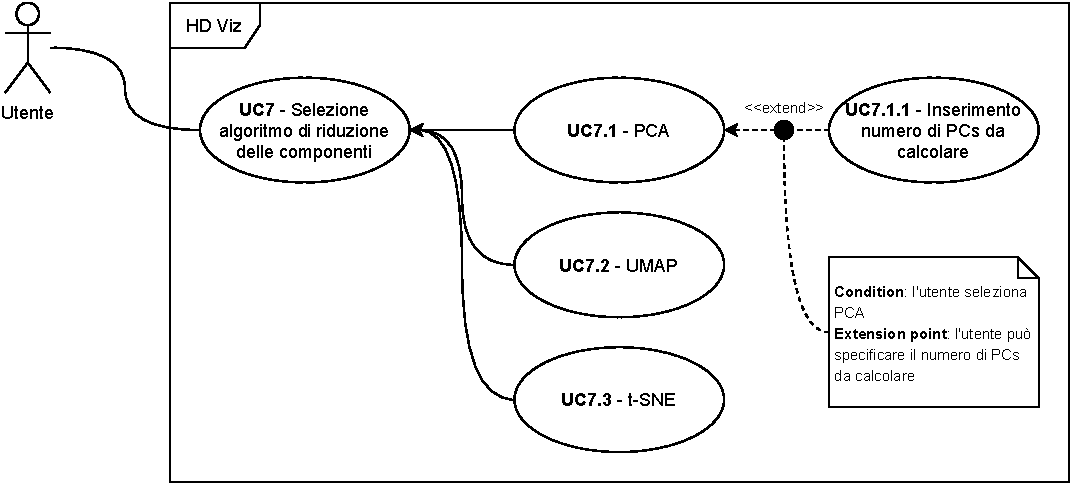
\includegraphics[width=0.9\textwidth]{source/sections/casi-uso/diagrams/uc7.pdf}
        \caption{UC7 - Selezione algoritmo di riduzione delle componenti}
        \label{fig:uc7}
    \end{figure}
    
    \begin{itemize}
    \item \textbf{Attore}: utente;
    \item \textbf{Descrizione}: l'utente sceglie l'algoritmo per la riduzione delle componenti per l'elaborazione dati;
    \item \textbf{Precondizione}: 
    \begin{itemize}
        \item eseguito l'upload del dataset come matrice $N\times M$ (\hyperref[uc1]{UC1});
        \item selezionato Linear Projection come visualizzazione \hyperref[uc2.5]{UC2.5}).
    \end{itemize}  
    \item \textbf{Postcondizione}: l'utente ha scelto l'algoritmo per la riduzione delle componenti;
    \item \textbf{Scenario Principale}: 
    \begin{enumerate}
        \item l'utente seleziona l'algoritmo per la riduzione delle componenti tra quelli disponibili.
    \end{enumerate}
    \item \textbf{Generalizzazioni}:
        \begin{enumerate}
            \item l'utente seleziona una delle seguenti distanze:
                \begin{enumerate}
                    \item PCA (\hyperref[uc7.1]{UC7.1});
                    \item UMAP (\hyperref[uc7.2]{UC7.2});
                    \item t-SNE (\hyperref[uc7.3]{UC7.3}).
                \end{enumerate}
        \end{enumerate}  
    \end{itemize}
    
    \subsubsection{UC7.1 - PCA}
    \label{uc7.1}
    \begin{itemize}
    \item \textbf{Attore}: utente;
    \item \textbf{Descrizione}: il PCA è una tecnica di riduzione dimensionale, cioè a partire da $n$ features ne calcola $k$ ($k$ fissato), queste nuove k feature approssimano meglio le $n$ features iniziali;
    \item \textbf{Precondizione}: 
    \begin{itemize}
        \item eseguito l'upload del dataset come matrice $N\times M$ (\hyperref[uc1]{UC1});
        \item selezionato Linear Projection come visualizzazione (\hyperref[uc2.5]{UC2.5}).
    \end{itemize}  
    \item \textbf{Postcondizione}: il dataset contiene k nuove colonne (dove $k$ è il numero di PCs che l'utente ha scelto di calcolare), che sono le $k$ proiezioni calcolate da PCA;
    \item \textbf{Scenario Principale}: 
    \begin{enumerate}
        \item l'utente sceglie di applicare l'algoritmo PCA sul dataset.
    \end{enumerate}  
    \item \textbf{Inclusioni}:
        \begin{enumerate}
            \item inserimento del numero di PCs da calcolare (\hyperref[uc7.1.1]{UC7.1.1}).
        \end{enumerate} 
    \end{itemize}
    
    \paragraph{UC7.1.1 - PCA - Inserimento numero di PCs da calcolare}
    \label{uc7.1.1}
    \begin{itemize}
    \item \textbf{Attore}: utente;
    \item \textbf{Descrizione}: l'utente specifica quante nuove features il PCA deve calcolare;
    \item \textbf{Precondizione}: 
    \begin{itemize}
        \item eseguito l'upload del dataset come matrice $N\times M$ (\hyperref[uc1]{UC1});
        \item selezionato Linear Projection come visualizzazione (\hyperref[uc2.5]{UC2.5});
        \item selezionato PCA (\hyperref[uc7.1]{UC7.1}).
    \end{itemize}  
    \item \textbf{Postcondizione}: il numero k di features da calcolare è stato inserito;
    \item \textbf{Scenario Principale}: 
    \begin{enumerate}
        \item l'utente inserisce un numero k compreso tra 1 e il numero di features.
    \end{enumerate}  
    \end{itemize}
    
    \subsubsection{UC7.2 - UMAP}
    \label{uc7.2}
    \begin{itemize}
    \item \textbf{Attore}: utente;
    \item \textbf{Descrizione}: UMAP è una tecnica di riduzione dimensionale, cioè a partire da $n$ features ne calcola $k$ ($k$ fissato), queste nuove k feature approssimano meglio le $n$ features iniziali;
    \item \textbf{Precondizione}: 
    \begin{itemize}
        \item eseguito l'upload del dataset come matrice $N\times M$ (\hyperref[uc1]{UC1});
        \item selezionato Linear Projection come visualizzazione (\hyperref[uc2.5]{UC2.5}).
    \end{itemize}  
    \item \textbf{Postcondizione}: l'utente seleziona UMAP come algoritmo per la riduzione dimensionale;
    \item \textbf{Scenario Principale}: 
    \begin{enumerate}
        \item l'utente sceglie di applicare l'algoritmo UMAP sul dataset.
    \end{enumerate}
    \end{itemize}
    
    \subsubsection{UC7.3 - t-SNE}
    \label{uc7.3}
    \begin{itemize}
    \item \textbf{Attore}: utente;
    \item \textbf{Descrizione}: t-SNE è una tecnica di riduzione dimensionale, cioè a partire da $n$ features ne calcola $k$ ($k$ fissato), queste nuove k feature approssimano meglio le $n$ features iniziali;
    \item \textbf{Precondizione}: 
    \begin{itemize}
        \item eseguito l'upload del dataset come matrice $N\times M$ (\hyperref[uc1]{UC1});
        \item selezionato Linear Projection come visualizzazione (\hyperref[uc2.5]{UC2.5}).
    \end{itemize}  
    \item \textbf{Postcondizione}: l'utente seleziona t-SNE come algoritmo per la riduzione dimensionale;
    \item \textbf{Scenario Principale}: 
    \begin{enumerate}
        \item l'utente sceglie di applicare l'algoritmo t-SNE sul dataset.
    \end{enumerate}
    \end{itemize}
    
    

    \pagebreak
    \subsection{UC8 - Elaborazione dati}
    \label{uc8}
    \begin{itemize}
    \item \textbf{Attore}: Utente
    \item \textbf{Descrizione}: Vengono elaborati i dati secondo le impostazioni
    \item \textbf{Precondizione}: 
    \begin{itemize}
        \item Eseguito l'upload del dataset come matrice $N\times M$ (\hyperref[uc1]{UC1}).
        \item Selezionato un tipo di visualizzazione (\hyperref[uc2]{UC2}).
    \end{itemize}  
    \item \textbf{Postcondizione}: L'applicazione dopo che l'utente ha caricato il suo dataset e selezionato il tipo di visualizzazione, ha elaborato i dati secondo le impostazioni
    \item \textbf{Scenario Principale}: 
    \begin{enumerate}
        \item L'utente carica il suo dataset (\hyperref[uc1]{UC1})
        \item L'utente seleziona il tipo di visualizzazione tra quelle disponibili (\hyperref[uc2]{UC2})
        \item L'applicazione elabora i dati con impostazioni di default (\hyperref[uc8.1]{UC8.1})
        \item L'utente cambia le impostazioni (\hyperref[uc3]{UC3} o \hyperref[uc4]{UC4} \hyperref[uc5]{UC5} o \hyperref[uc6]{UC6} o \hyperref[uc7]{UC7})
        \item L'applicazione rielabora i dati (\hyperref[uc8.2]{UC8.2})
    \end{enumerate}
    \end{itemize}
    
    % Nel caso di visualizzazioni che richiedono delle impostazioni obbligatorie? (esempio calcolare matrice di distanza prima di visualizzare il grafico force-field)
    \subsubsection{UC8.1 - Avvio elaborazione dati con impostazioni di default}
    \label{uc8.1}
    \begin{itemize}
    \item \textbf{Attore}: Utente
    \item \textbf{Descrizione}: L'utente avvia l'elaborazione dati secondo le impostazioni di deafult
    \item \textbf{Precondizione}: 
    \begin{itemize}
        \item Eseguito l'upload del dataset come matrice $N\times M$ (\hyperref[uc1]{UC1}).
        \item Selezionato un tipo di visualizzazione (\hyperref[uc2]{UC2}).
    \end{itemize}  
    \item \textbf{Postcondizione}: L'applicazione dopo che l'utente dopo ha caricato il suo dataset e selezionato il tipo di visualizzazione, ha avviato l'elaborazione dei dati secondo le impostazioni di default
    \item \textbf{Scenario Principale}: 
    \begin{enumerate}
        \item L'utente carica il suo dataset (\hyperref[uc1]{UC1})
        \item L'utente seleziona il tipo di visualizzazione tra quelle disponibili (\hyperref[uc2]{UC2})
        \item L'applicazione elabora i dati
    \end{enumerate}
    \end{itemize}
    
    \subsubsection{UC8.2 - Avvio elaborazione dati con impostazioni utente}
    \label{uc8.2}
    \begin{itemize}
    \item \textbf{Attore}: Utente
    \item \textbf{Descrizione}:  L'utente avvia l'elaborazione dati secondo le impostazioni personalizzate
    \item \textbf{Precondizione}: 
    \begin{itemize}
        \item Eseguito l'upload del dataset come matrice $N\times M$ (\hyperref[uc1]{UC1}).
        \item Selezionato un tipo di visualizzazione (\hyperref[uc2]{UC2}).
        \item L'utente ha cambiato le impostazioni (\hyperref[uc3]{UC3} o \hyperref[uc4]{UC4} \hyperref[uc5]{UC5} o \hyperref[uc6]{UC6} o \hyperref[uc7]{UC7})
    \end{itemize}  
    \item \textbf{Postcondizione}: L'applicazione dopo che l'utente ha caricato il suo dataset e selezionato il tipo di visualizzazione, ha avviato l'elaborazione dei dati secondo le impostazioni personalizzate inserite dall'utente
    \item \textbf{Scenario Principale}: 
    \begin{enumerate}
        \item L'utente carica il suo dataset (\hyperref[uc1]{UC1})
        \item L'utente seleziona il tipo di visualizzazione tra quelle disponibili (\hyperref[uc2]{UC2})
        \item L'applicazione elabora i dati (\hyperref[uc8.1]{UC8.1})
        \item L'utente cambia le impostazioni (\hyperref[uc3]{UC3} o \hyperref[uc4]{UC4} \hyperref[uc5]{UC5} o \hyperref[uc6]{UC6} o \hyperref[uc7]{UC7})
        \item L'applicazione rielabora i dati
    \end{enumerate}
    \end{itemize}